%%%%%%%%%%%%%%%%%%%%%%%%%%%%%%%%%%%%%%%%%%%
%%%%%%%%%%%%%%%%%%%%%%%%%%%%%%%%%%%%%%%%%%%
%%%%%%%%%%%%%%% CHAPTER 09 %%%%%%%%%%%%%%%%


\section{Diagrama de blocos}

\frame{
\frametitle{Introdução}
\begin{block}{Contextualização}
Estivemos trabalhando com subsistemas individuais representados por um bloco com sua entrada e sua saída. Entretanto, sistemas mais \textbf{complexos} são representados pela \textbf{interconexão de diversos subsistemas}.
\end{block}
}

\frame{
\frametitle{Introdução}
\begin{block}{Definição}
Um \textbf{diagrama de blocos} de um sistema é uma representação \textbf{gráfica} das funções desempenhadas por cada componente e o fluxo de sinais entre eles.
\begin{itemize}
    \item Diferindo da representação matemática pura, um diagrama de blocos tem a vantagem de indicar mais \textbf{realisticamente} o fluxo de sinais do sistema real.
\end{itemize}
\end{block}
}

\frame{
\frametitle{Introdução}
\begin{block}{Bloco}
Em um \textbf{diagrama de blocos}, todas as variáveis do sistema são ligadas uma as outras por meio de blocos funcionais, ou simplesmente \textbf{bloco}.
\begin{itemize}
    \item O bloco é um símbolo da operação matemática que é aplicado ao sinal de \textbf{entrada} e que produz o sinal de \textbf{saída}. A função de transferência dos componentes é normalmente incluída nos blocos correspondentes, os quais são indicados por setas. As setas também indicam a direção do fluxo do sinal.
\end{itemize}
\end{block}
\vspace{0.2cm}
\centerline{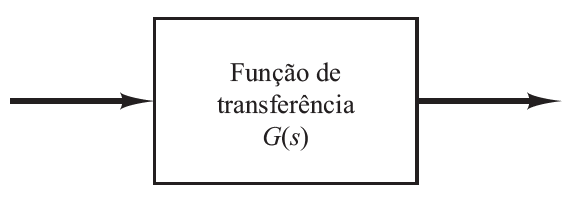
\includegraphics[width=0.5\linewidth]{Figuras/Ch09/fig1.PNG}}
}

\frame{
\frametitle{Componentes de um diagrama de blocos}
\begin{block}{Sinais}
A seta que aponta para o bloco indica a \textbf{entrada} e a seta que aponta para fora do bloco representa a \textbf{saída}. Essas setas são designadas como \textbf{sinais}.
\end{block}
\vspace{0.2cm}
\centerline{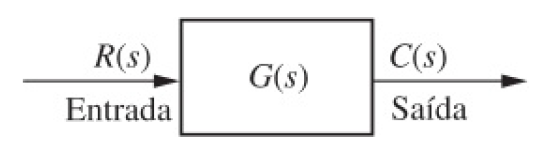
\includegraphics[width=0.5\linewidth]{Figuras/Ch09/fig2.PNG}}
}

\frame{
\frametitle{Componentes de um diagrama de blocos}
\begin{block}{Junção de soma}
Um círculo com uma cruz é o símbolo que indica a operação de \textbf{soma}. O sinal de mais ou menos na extremidade de cada seta indica se o sinal deve ser \textbf{somado} ou \textbf{subtraído}.
\begin{itemize}
    \item É importante que as quantidades a serem somadas ou subtraídas tenham as mesmas dimensões e as mesmas unidades.
\end{itemize}
\end{block}
\vspace{0.2cm}
\centerline{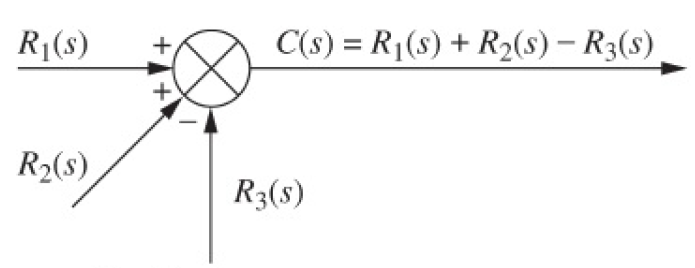
\includegraphics[width=0.6\linewidth]{Figuras/Ch09/fig3.PNG}}
}

\frame{
\frametitle{Componentes de um diagrama de blocos}
\begin{block}{Ponto de ramificação}
Um \textbf{ponto de ramificação} é um ponto do qual o sinal que vem de um bloco \textbf{avança simultaneamente} em direção a outros blocos ou somadores.
\end{block}
\vspace{0.2cm}
\centerline{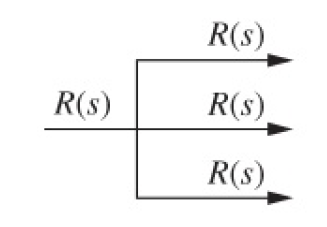
\includegraphics[width=0.4\linewidth]{Figuras/Ch09/fig4.PNG}}
}

\frame{
\frametitle{Topologias comuns para interconectar subsistemas}
\begin{block}{Cascata}
Nesta configuração, valores de \textbf{sinais intermediários} são mostrados na saída de cada subsistema.
\begin{itemize}
    \item Cada sinal é obtido pelo \textbf{produto da entrada pela função de transferência}.
\end{itemize}
$$G_e(s) = G_3(s)G_2(s)G_1(s)$$
\end{block}
\vspace{0.2cm}
\centerline{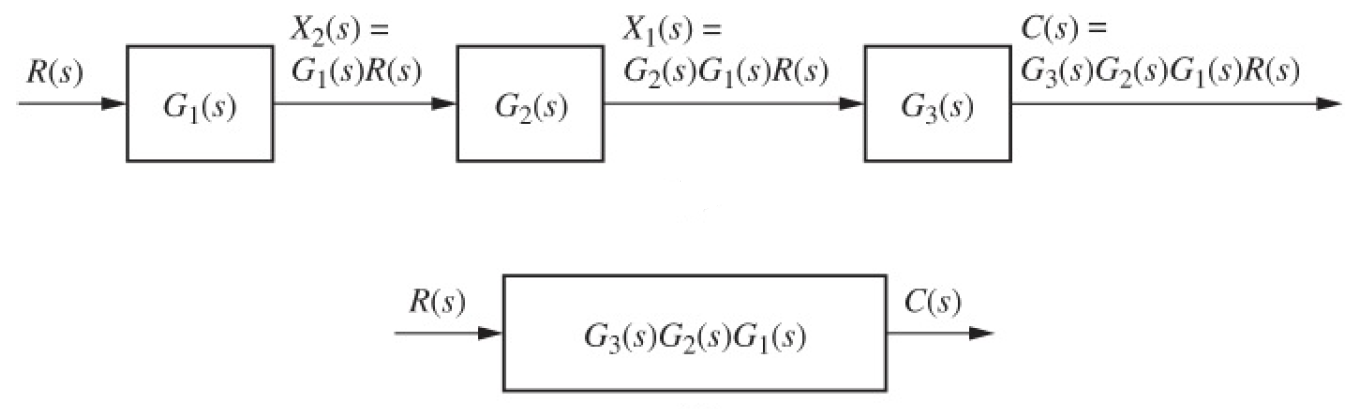
\includegraphics[width=1.1\linewidth]{Figuras/Ch09/fig5.PNG}}
}

\frame{
\frametitle{Topologias comuns para interconectar subsistemas}
\begin{block}{Paralelo}
Os subsistemas em paralelo possuem uma \textbf{entrada comum} e uma saída formada pela soma algébrica das saídas de todos os subsistemas.
\begin{itemize}
    \item Cada sinal é obtido pelo \textbf{produto da entrada (comum a todos os blocos) pela função de transferência}.
\end{itemize}
$$G_e(s) = \pm G_1(s) \pm G_2(s) \pm G_3(s)$$
\end{block}
\vspace{0.2cm}
\centerline{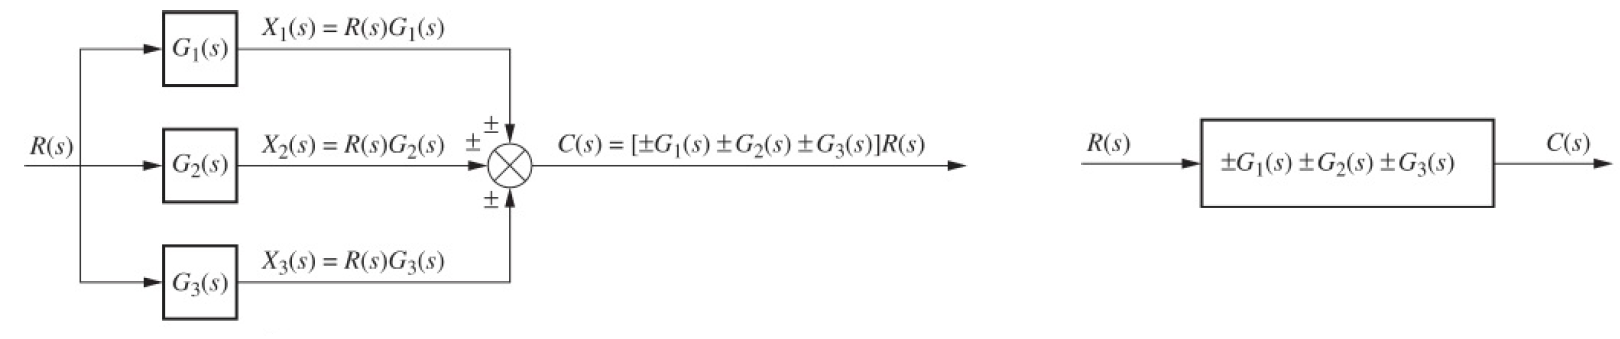
\includegraphics[width=1.15\linewidth]{Figuras/Ch09/fig6.PNG}}
}

\frame{
\frametitle{Topologias comuns para interconectar subsistemas}
\begin{block}{Realimentação}
O sistema com \textbf{realimentação} forma a base para nosso estudo da engenharia de sistemas de controle.
\begin{itemize}
    \item Antes de prosseguirmos com essa topologia, precisamos definir o que é um sistema em \textbf{malha aberta} e o que é um sistema em \textbf{malha fechada}.
\end{itemize}
\end{block}
}

\frame{
\frametitle{Configurações de sistemas}
\begin{block}{Sistemas em malha aberta}
\begin{itemize}
    \item O \textbf{transdutor de entrada} converte a forma de entrada para aquela utilizada pelo \textbf{controlador}.
    \item O controlador aciona um processo ou uma \textbf{planta}.
    \item A entrada algumas vezes é chamada de \textbf{referência}, enquanto a saída pode ser chamada de \textbf{variável controlada}.
\end{itemize}
\end{block}
\vspace{0.2cm}
\centerline{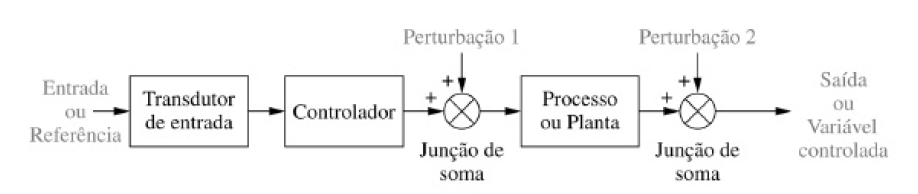
\includegraphics[width=1.15\linewidth]{Figuras/Ch09/fig7.PNG}}
}

\frame{
\frametitle{Configurações de sistemas}
\begin{block}{Sistemas em malha aberta}
\begin{itemize}
    \item A característica distintiva de um sistema em malha aberta é que ele \textbf{não pode realizar compensações para quaisquer pertubações} que sejam adicionadas ao sinal de acionamento do controlador. 
    \item A saída de um sistema em malha aberta é corrompida não apenas por sinais que são adicionados aos comandos do controlador, mas também por \textbf{pertubações na saída}.
    \item Estes sistemas são comandados simplesmente pela \textbf{entrada}.
    \item \textbf{Exemplo}: a torradeira elétrica é um sistema em malha aberta - o aparelho \textbf{não mede} a cor da torrada e não efetua correções se o pão possuir ingredientes ou espessuras diferentes.
\end{itemize}
\end{block}
\vspace{0.2cm}
}

\frame{
\frametitle{Configurações de sistemas}
\begin{block}{Sistemas em malha fechada}
\begin{itemize}
    \item O \textbf{transdutor de entrada} converte a forma de entrada para aquela utilizada pelo \textbf{controlador}.
    \item Um transdutor de saída, ou \textbf{sensor}, mede a resposta da saída e a converte para a forma utilizada pelo controlador.
    \item Suponha que o controlador utilize \textbf{sinais elétricos} para operar as válvulas de um sistema de temperatura. A posição de entrada pode ser convertida em tensão por meio de um \textbf{potenciômetro}, e a temperatura de saída pode ser convertida por meio de um \textbf{termistor}.
\end{itemize}
\end{block}
\centerline{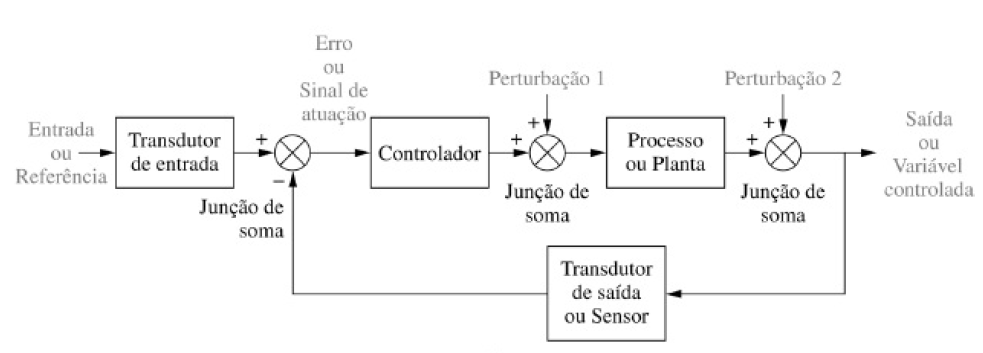
\includegraphics[width=0.76\linewidth]{Figuras/Ch09/fig8.PNG}}
}

\frame{
\frametitle{Configurações de sistemas}
\begin{block}{Sistemas em malha fechada}
\begin{itemize}
    \item O sinal de saída, que chega através da \textbf{malha de realimentação}, é subtraído do sinal de entrada. O resultado, geralmente, é chamado de \textbf{sinal de atuação}. Em sistemas em que ambos os transdutores possuem ganho unitário, o sinal de atuação é chamado de \textbf{erro}.
    \item O sistema em malha fechada compensa o efeito das pertubações \textbf{medindo a resposta} da saída, \textbf{realimentando} essa medida através da malha de realimentação e \textbf{comparando} essa resposta com a entrada na junção de soma.
\end{itemize}
\end{block}
\centerline{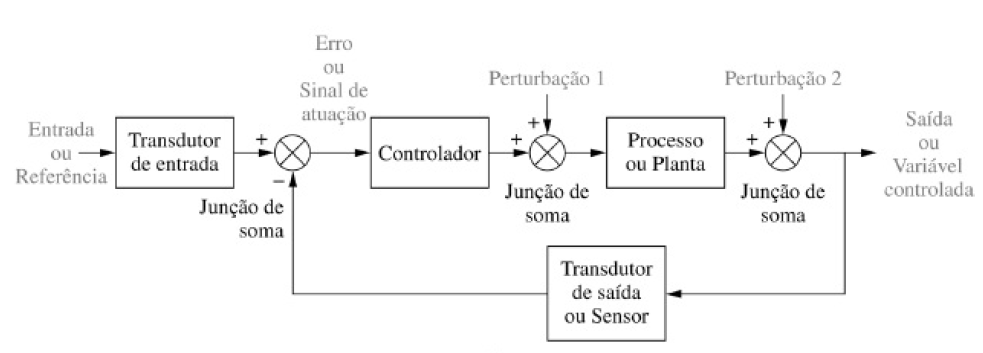
\includegraphics[width=0.78\linewidth]{Figuras/Ch09/fig8.PNG}}
}

\frame{
\frametitle{Configurações de sistemas}
\begin{block}{Sistemas em malha fechada}
\begin{itemize}
    \item Assim, os sistemas em malha fechada possuem a vantagem óbvia de apresentar uma \textbf{exatidão} maior que os sistemas em malha aberta.
    \item Eles são \textbf{menos sensíveis} a ruídos, pertubações e alterações do ambiente.
    \item Por outro lado, estes são \textbf{mais complexos e mais caros} que sistemas em malha aberta.
    \item \textbf{Exemplo}: uma torradeira de forno em malha fechada é mais complexa e mais cara, uma vez que ela tem que \textbf{medir} tanto a cor (por meio da reflexão de luz) quanto a umidade em seu interior.
    \item Papel do \textbf{engenheiro}: analisar o \textit{tradeoff}.
\end{itemize}
\end{block}
}

\frame{
\frametitle{Topologias comuns para interconectar subsistemas}
\begin{block}{Realimentação}
Agora poderemos deduzir a \textbf{função de transferência} de um sistema de controle com \textbf{realimentação} (sistema em malha fechada).
\end{block}
\vspace{0.2cm}
\centerline{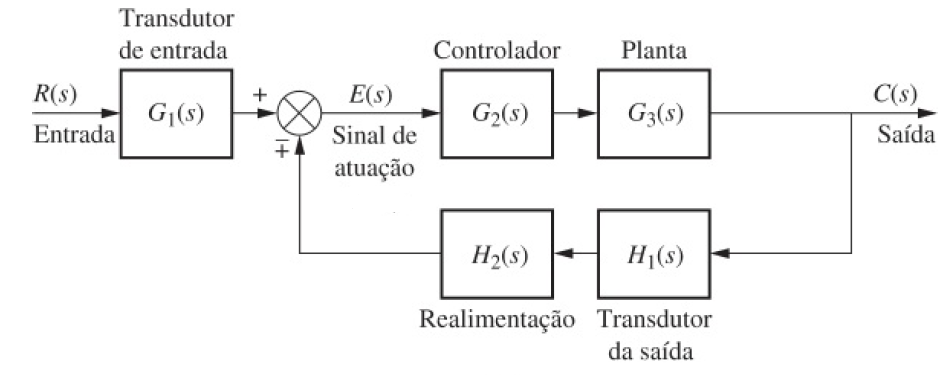
\includegraphics[width=0.9\linewidth]{Figuras/Ch09/fig9.PNG}}
}

\frame{
\frametitle{Topologias comuns para interconectar subsistemas}
\begin{block}{Realimentação}
Considere o \textbf{modelo simplificado} abaixo.
\begin{itemize}
    \item O sinal de \textbf{erro} é dado por
    $$E(s) = R(s) \mp C(s)H(s)$$
    \item Mas, uma vez que $C(s) = E(s)G(s)$,
    $$E(s) = \dfrac{C(s)}{G(s)}$$
\end{itemize}
\end{block}
\centerline{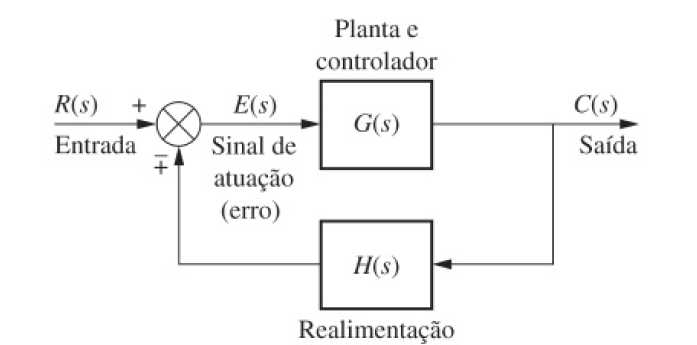
\includegraphics[width=0.53\linewidth]{Figuras/Ch09/fig10.PNG}}
}

\frame{
\frametitle{Topologias comuns para interconectar subsistemas}
\begin{block}{Realimentação}
\begin{itemize}
    \item Substituindo, obtemos:
\end{itemize}
$$\dfrac{C(s)}{G(s)} = R(s) \mp C(s)H(s)$$
$$C(s) = G(s)R(s) \mp G(s)C(s)H(s)$$
$$C(s) \pm G(s)C(s)H(s) = G(s)R(s)$$
$$C(s)[1 \pm G(s)H(s)] = G(s)R(s)$$
$$\boxed{\dfrac{C(s)}{R(s)} = \dfrac{G(s)}{1 \pm G(s)H(s)}}$$
que é definida como a \textbf{função de transferência de malha fechada}.
\end{block}
}

\frame{
\frametitle{Topologias comuns para interconectar subsistemas}
\begin{block}{Realimentação}
\begin{itemize}
    \item Definimos ainda:
\end{itemize}
$$\boxed{\dfrac{B(s)}{E(s)} = G(s)H(s)}$$
que é definida como a \textbf{função de transferência de malha aberta}, que relaciona o sinal de realimentação $B(s)$ e o sinal de erro atuante $E(s)$.
\vspace{0.4cm}
\begin{itemize}
    \item Além disso:
\end{itemize}
$$\boxed{\dfrac{C(s)}{E(s)} = G(s)}$$
que é definida como a \textbf{função de transferência do ramo direto}, que relaciona o sinal de saída $C(s)$ e o sinal de erro atuante $E(s)$.
\end{block}
}

\cprotect\frame{
\frametitle{\MATLAB}
\begin{block}{}
\begin{verbatim}
>>[num,den] = series(num1,den1,num2,den2)
\end{verbatim}
retorna a função de transferência de um sistema em cascata. \\
\end{block}
\centerline{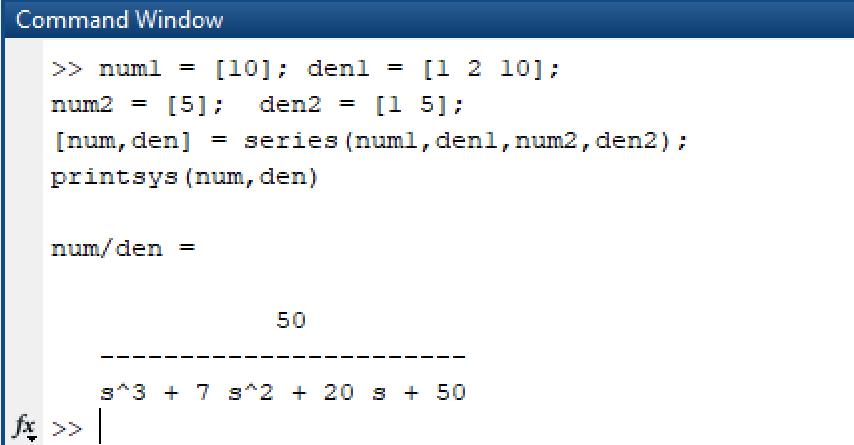
\includegraphics[width=0.75\linewidth]{Figuras/Ch09/fig11.PNG}}
}

\cprotect\frame{
\frametitle{\MATLAB}
\begin{block}{}
\begin{verbatim}
>>[num,den] = parallel(num1,den1,num2,den2)
\end{verbatim}
retorna a função de transferência de um sistema em paralelo. \\
\end{block}
\centerline{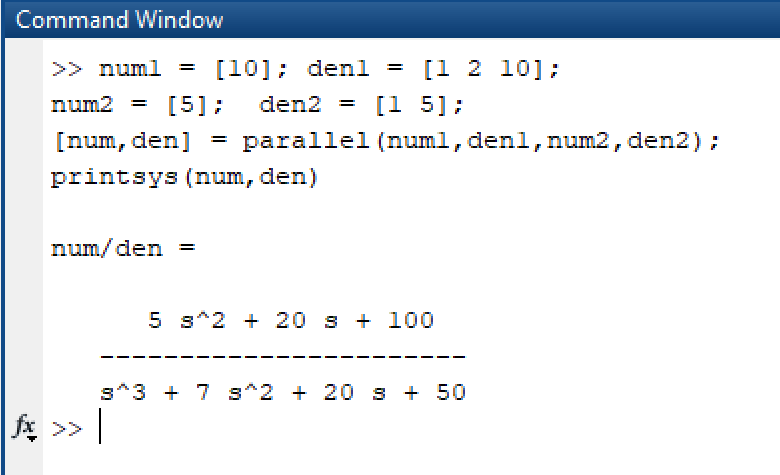
\includegraphics[width=0.7\linewidth]{Figuras/Ch09/fig12.PNG}}
}

\cprotect\frame{
\frametitle{\MATLAB}
\begin{block}{}
\begin{verbatim}
>>[num,den] = feedback(num1,den1,num2,den2)
\end{verbatim}
retorna a função de transferência de um sistema com realimentação. \\
\end{block}
\centerline{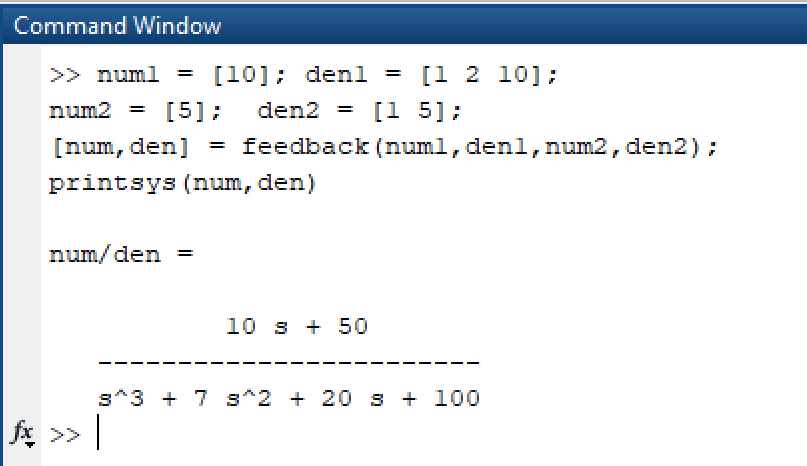
\includegraphics[width=0.7\linewidth]{Figuras/Ch09/fig13.PNG}}
}

\frame{
\frametitle{Exemplo $\#01$ - realimentação unitária negativa}
\begin{block}{}
Obtenha a função de transferência de malha fechada para $$G(s) = \dfrac{10}{s^2+5s+20} \ \text{e} \ H(s) = 1$$

\vspace{0.2cm}

\textbf{Solução}: Quando $H(s) = 1$ dizemos que este sistema possui realimentação unitária. Uma forma alternativa (no caso de realimentação negativa) à fórmula
$$\dfrac{C(s)}{R(s)} = \dfrac{G(s)}{1 + G(s)H(s)}$$
é simplesmente dizer que a função de transferência de malha fechada é igual a $G(s)$, acrescentando no denominador o próprio numerador de $G(s)$. Deste modo,
$$\dfrac{C(s)}{R(s)} = \dfrac{\bm{10}}{s^2+5s+20\bm{+10}} = \dfrac{10}{s^2+5s+30}$$
\end{block}
}

\frame{
\frametitle{Sistema de malha fechada submetido a um distúrbio}
\begin{block}{Função de transferência}
Quando \textbf{duas entradas} (a entrada de \textbf{referência} e o \textbf{distúrbio}) estão presentes em um SLIT, cada entrada pode ser tratada \textbf{independente} da outra e as saídas que correspondem a cada entrada individual podem ser somadas para resultar na saída completa.
\begin{itemize}
    \item Fazendo $D(s) = 0$:
\end{itemize}
$$\dfrac{C_R(s)}{R(s)} = \dfrac{G_1(s)G_2(s)}{1 + G_1(s)G_2(s)H(s)}$$
\end{block}
\vspace{0.2cm}
\centerline{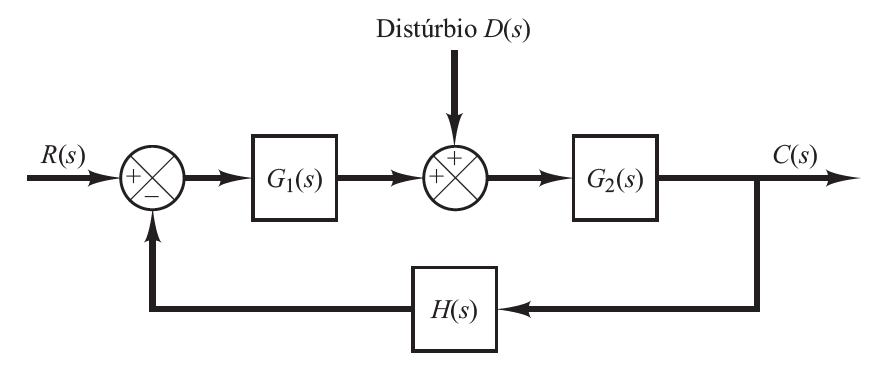
\includegraphics[width=0.65\linewidth]{Figuras/Ch09/fig14.PNG}}
}

\frame{
\frametitle{Sistema de malha fechada submetido a um distúrbio}
\begin{block}{Função de transferência}
\begin{itemize}
    \item Fazendo $R(s) = 0$:
\end{itemize}
$$\dfrac{C_D(s)}{D(s)} = \dfrac{G_2(s)}{1 + G_1(s)G_2(s)H(s)}$$
\end{block}
\vspace{0.2cm}
\centerline{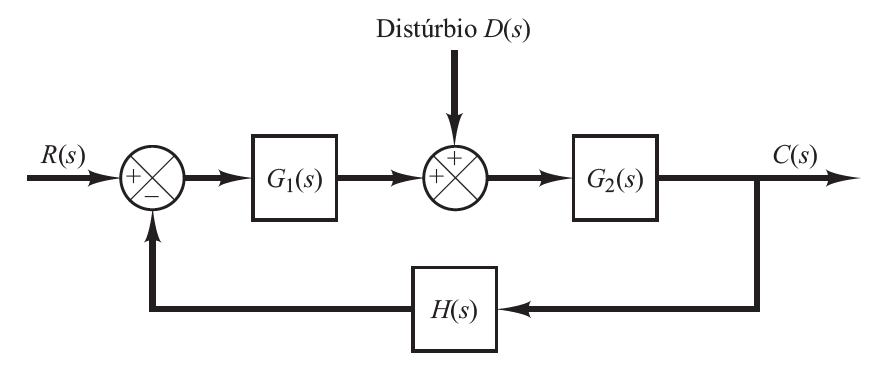
\includegraphics[width=0.7\linewidth]{Figuras/Ch09/fig14.PNG}}
}

\frame{
\frametitle{Procedimento para construir um diagrama de blocos}
\begin{block}{Passos necessários}
\begin{enumerate}
    \item Realize a \textbf{modelagem matemática} do sistema proposto.
    \item Resolva a EDO para a \textbf{maior ordem da derivada} da variável de saída desconhecida.
    \item Conecte um ou mais \textbf{blocos integradores em série} com o objetivo de integrar tal derivada de forma sucessiva quantas vezes forem necessárias, até chegar na variável de saída.
    \item Use o resultado do passo 2 para representar a maior ordem da derivada como uma \textbf{saída de blocos de soma e ganho}.
\end{enumerate}
\end{block}
}

\frame{
\frametitle{Exemplo $\#02$ - sistema massa-mola-amortecedor}
\centerline{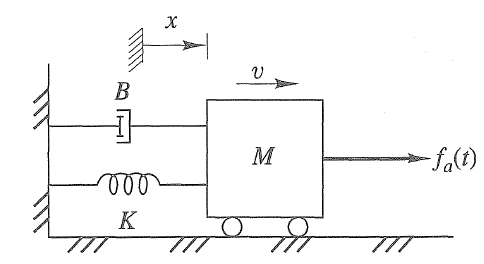
\includegraphics[width=0.5\linewidth]{Figuras/Ch05/fig8.PNG}}
\begin{block}{Procedimento para construir um diagrama de blocos}
\begin{itemize}
    \item O primeiro passo (modelagem matemática) já foi realizado em capítulos anteriores:
\end{itemize}
$$M\ddot{x} + B\dot{x} + Kx = f_a(t)$$
\begin{itemize}
    \item O passo 2 consiste em isolar $\ddot{x}$:
\end{itemize}
$$\ddot{x} = \dfrac{1}{M}[f_a(t)- B\dot{x} - Kx]$$
\end{block}
}

\frame{
\frametitle{Exemplo $\#02$ - sistema massa-mola-amortecedor}
\begin{block}{Procedimento para construir um diagrama de blocos}
\begin{itemize}
    \item O terceiro passo consiste em usar dois integradores (já que a ordem da maior derivada é 2) para relacionar $\ddot{x}$, $\dot{x}$ e $x$.
\end{itemize}
\end{block}
\centerline{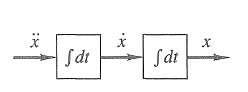
\includegraphics[width=0.5\linewidth]{Figuras/Ch09/fig15.PNG}}
}

\frame{
\frametitle{Exemplo $\#02$ - sistema massa-mola-amortecedor}
\begin{block}{Procedimento para construir um diagrama de blocos}
\begin{itemize}
    \item O último passo consiste em somar as três parcelas que dão origem a $\ddot{x}$ (vide passo 2), que são $f_a(t)$, $B\dot{x}$ e $Kx$. O diagrama de blocos completo é mostrado logo abaixo.
\end{itemize}
\end{block}
\centerline{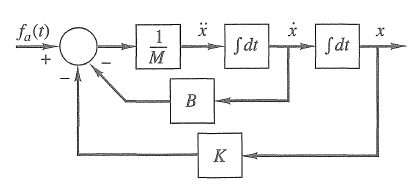
\includegraphics[width=0.7\linewidth]{Figuras/Ch09/fig16.PNG}}
}

\frame{
\frametitle{Exemplo $\#03$ - sistema com duas massas interconectadas}
\centerline{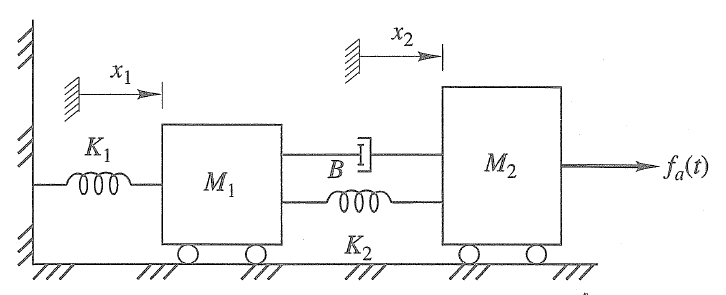
\includegraphics[width=0.5\linewidth]{Figuras/Ch05/fig10.PNG}}
\vspace{-0.2cm}
\begin{block}{Procedimento para construir um diagrama de blocos}
\begin{itemize}
    \item O primeiro passo (modelagem matemática) já foi realizado em capítulos anteriores:
\end{itemize}
\begin{equation*}
\begin{cases}
M_1\ddot{x}_1 + B\dot{x}_1 + (K_1 + K_2)x_1 - B\dot{x}_2 - K_2x_2= 0 \\
-B\dot{x}_1 - K_2x_1 + M_2\ddot{x}_2 + B\dot{x}_2 + K_2x_2 = f_a(t)
\end{cases}
\end{equation*}
\begin{itemize}
    \item O passo 2 consiste em isolar $\ddot{x}_1$ e $\ddot{x}_2$:
\end{itemize}
\begin{equation*}
\begin{cases}
\ddot{x}_1 = \dfrac{1}{M_1}[-B\dot{x}_1 - (K_1 + K_2)x_1 + B\dot{x}_2 + K_2x_2] \\
\ddot{x}_2 = \dfrac{1}{M_2}[f_a(t) - B\dot{x}_2 +B\dot{x}_1 - K_2x_2 + K_2x_1]
\end{cases}
\end{equation*}
\end{block}
}

\frame{
\frametitle{Exemplo $\#03$ - sistema com duas massas interconectadas}
\begin{block}{Procedimento para construir um diagrama de blocos}
\begin{itemize}
    \item O terceiro passo consiste em usar dois integradores (já que a ordem da maior derivada é 2) para relacionar $\ddot{x}_1$, $\dot{x}_1$ e $x_1$; e mais dois integradores para relacionar $\ddot{x}_2$, $\dot{x}_2$ e $x_2$, separadamente.
    \item O último passo consiste em somar as quatro parcelas que dão origem a $\ddot{x}_1$ (vide passo 2), além de somar as cinco parcelas que dão origem a $\ddot{x}_2$ (vide passo 2)
\end{itemize}
\end{block}
}

\frame{
\frametitle{Exemplo $\#03$ - sistema com duas massas interconectadas}
\centerline{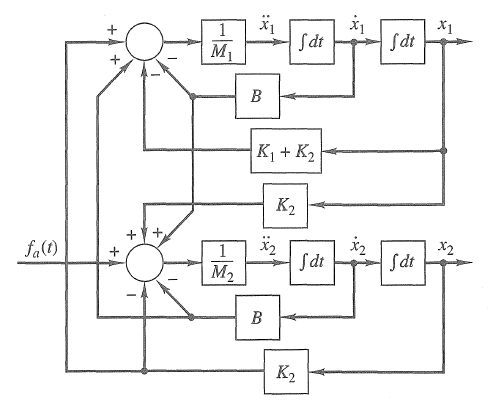
\includegraphics[width=0.8\linewidth]{Figuras/Ch09/fig17.PNG}}
}

\frame{
\frametitle{Redução de diagrama de blocos}
\begin{block}{Contextualização}
As formas familiares (em cascata, paralela e com realimentação) nem sempre ficam \textbf{aparentes} em um diagrama de blocos.
\begin{itemize}
    \item Se por exemplo na forma com realimentação houver um ponto de ramificação depois da junção de soma, não é possível utilizar a fórmula aprendida. 
\end{itemize}
\end{block}
}

\frame{
\frametitle{Redução de diagrama de blocos}
\begin{block}{Definição}
Iremos estudar agora \textbf{movimentos básicos de blocos} que podem ser feitos com a finalidade de estabelecer formas familiares quando elas quase existirem.
\begin{itemize}
    \item Em particular, será explicado como \textbf{mover os blocos} para a esquerda e para direita passando por \textbf{junções de soma e pontos de ramificação}.
\end{itemize}
\end{block}
}

\frame{
\frametitle{Redução de diagrama de blocos}
\begin{block}{Álgebra de diagrama de blocos para junções de soma}
\begin{itemize}
    \item Bloco movendo para a \textbf{esquerda}, passando por uma junção de soma.
    \item $C(s) = [R(s) \mp X(s)]G(s)$
    \item $C(s) = R(s)G(s) \mp X(s)G(s)$
\end{itemize}
\end{block}
\vspace{0.4cm}
\centerline{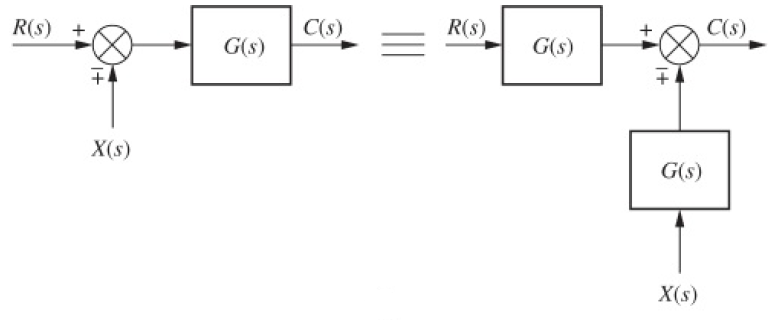
\includegraphics[width=0.8\linewidth]{Figuras/Ch09/fig18.PNG}}
}

\frame{
\frametitle{Redução de diagrama de blocos}
\begin{block}{Álgebra de diagrama de blocos para junções de soma}
\begin{itemize}
    \item Bloco movendo para a \textbf{direita}, passando por uma junção de soma.
    \item $C(s) = R(s)G(s) \mp X(s)$
    \item $C(s) = [R(s) \mp X(s) \dfrac{1}{G(s)}] G(s)$
\end{itemize}
\end{block}
\vspace{0.4cm}
\centerline{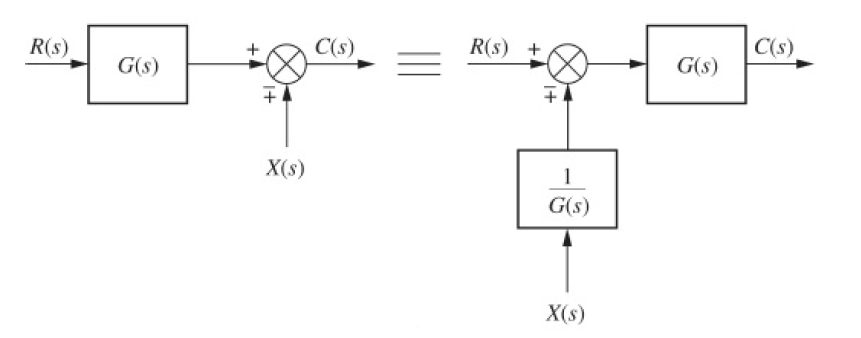
\includegraphics[width=0.9\linewidth]{Figuras/Ch09/fig19.PNG}}
}

\frame{
\frametitle{Redução de diagrama de blocos}
\begin{block}{Álgebra de diagrama de blocos para pontos de ramificação}
\begin{itemize}
    \item Bloco movendo para a \textbf{esquerda}, passando por um ponto de ramificação.
\end{itemize}
\end{block}
\vspace{0.4cm}
\centerline{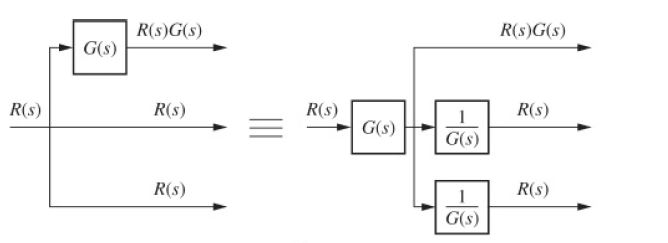
\includegraphics[width=0.9\linewidth]{Figuras/Ch09/fig20.PNG}}
}

\frame{
\frametitle{Redução de diagrama de blocos}
\begin{block}{Álgebra de diagrama de blocos para pontos de ramificação}
\begin{itemize}
    \item Bloco movendo para a \textbf{direita}, passando por um ponto de ramificação.
\end{itemize}
\end{block}
\vspace{0.4cm}
\centerline{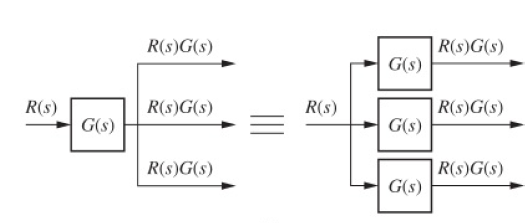
\includegraphics[width=0.8\linewidth]{Figuras/Ch09/fig21.PNG}}
}

\frame{
\frametitle{Exemplo $\#04$ - redução de diagrama de blocos}
\centerline{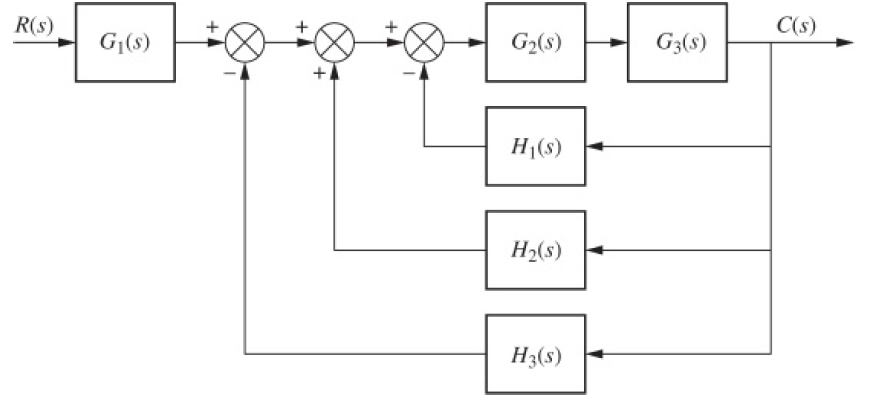
\includegraphics[width=1.1\linewidth]{Figuras/Ch09/fig22.PNG}}
}

\frame{
\frametitle{Exemplo $\#04$ - redução de diagrama de blocos}
\begin{block}{Resolução}
\begin{itemize}
    \item O primeiro passo é combinar as três junções de soma em uma única \textbf{junção de soma}.
\end{itemize}
\end{block}
\centerline{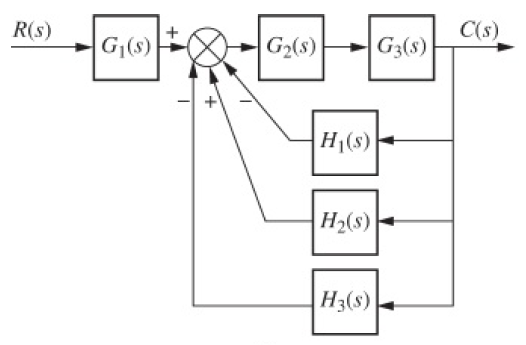
\includegraphics[width=0.7\linewidth]{Figuras/Ch09/fig23.PNG}}
}

\frame{
\frametitle{Exemplo $\#04$ - redução de diagrama de blocos}
\begin{block}{Resolução}
\begin{itemize}
    \item Após isso, deve-se perceber que as três funções de realimentação, $H_1(s)$, $H_2(s)$ e $H_3(s)$, estão conectadas em \textbf{paralelo}. Elas são alimentadas a partir de uma fonte de sinal comum, e suas saídas são somadas.
    \item Perceba também que $G_2(s)$ e $G_3(s)$ estão conectadas em \textbf{cascata}.
\end{itemize}
\end{block}
\centerline{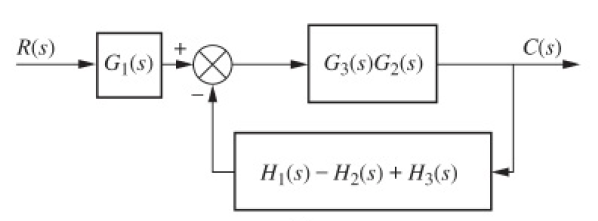
\includegraphics[width=0.7\linewidth]{Figuras/Ch09/fig24.PNG}}
}

\frame{
\frametitle{Exemplo $\#04$ - redução de diagrama de blocos}
\begin{block}{Resolução}
\begin{itemize}
    \item Finalmente, o sistema com \textbf{realimentação} é reduzido e multiplicado por $G_1(s)$.
\end{itemize}
\end{block}
\centerline{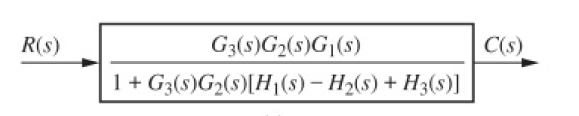
\includegraphics[width=0.7\linewidth]{Figuras/Ch09/fig25.PNG}}
}











\frame{
\frametitle{Exemplo $\#05$ - redução de diagrama de blocos}
\centerline{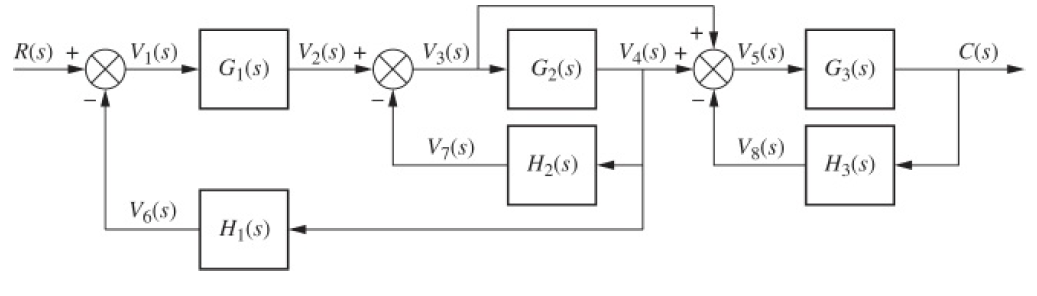
\includegraphics[width=1.1\linewidth]{Figuras/Ch09/fig26.PNG}}
}

\frame{
\frametitle{Exemplo $\#05$ - redução de diagrama de blocos}
\begin{block}{Resolução}
\begin{itemize}
    \item O primeiro passo é mover $G_2(s)$ para a esquerda passando o ponto de ramificação, com o objetivo de criar subsistemas \textbf{paralelos}.
    \item Além disso, podemos reduzir o sistema $G_3(s)$ e $H_3(s)$ por meio da \textbf{realimentação}.
\end{itemize}
\end{block}
\vspace{0.3cm}
\centerline{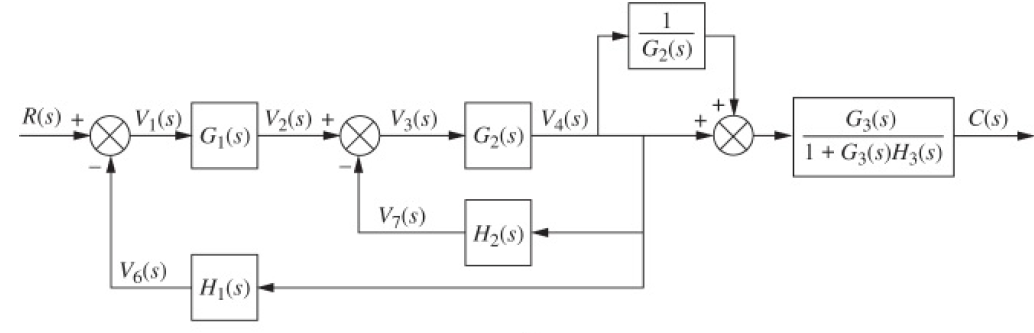
\includegraphics[width=1.1\linewidth]{Figuras/Ch09/fig27.PNG}}
}

\frame{
\frametitle{Exemplo $\#05$ - redução de diagrama de blocos}
\begin{block}{Resolução}
\begin{itemize}
    \item Após isso, o par paralelo pode ser \textbf{somado}.
    \item O bloco $G_1(s)$ pode ser movido para a direita passando a \textbf{junção de soma}, criando subsistemas paralelos na realimentação.
\end{itemize}
\end{block}
\vspace{0.3cm}
\centerline{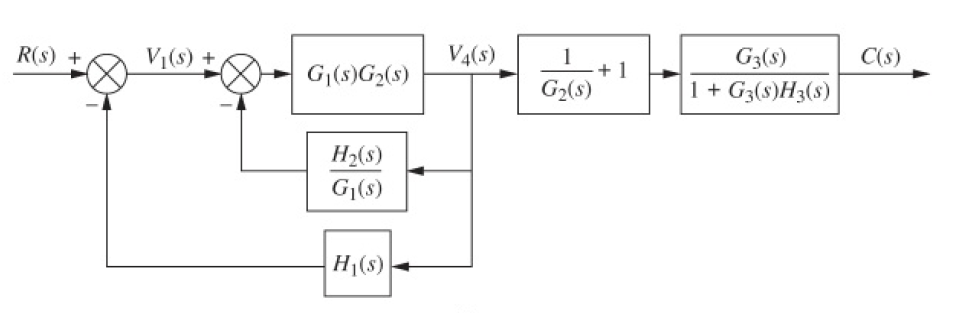
\includegraphics[width=1.1\linewidth]{Figuras/Ch09/fig28.PNG}}
}

\frame{
\frametitle{Exemplo $\#05$ - redução de diagrama de blocos}
\begin{block}{Resolução}
\begin{itemize}
    \item \textbf{Combine} as junções de soma, somando os dois elementos da realimentação.
    \item Combine os dois últimos blocos em \textbf{cascata}.
\end{itemize}
\end{block}
\vspace{0.3cm}
\centerline{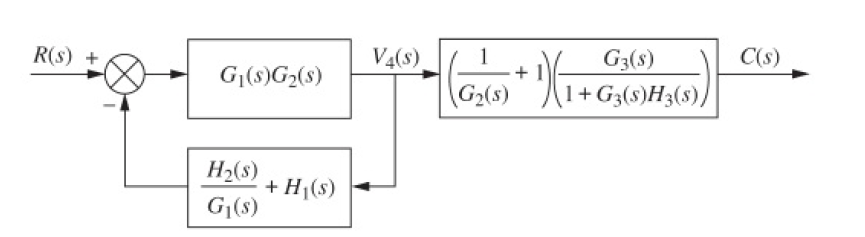
\includegraphics[width=1.1\linewidth]{Figuras/Ch09/fig29.PNG}}
}

\frame{
\frametitle{Exemplo $\#05$ - redução de diagrama de blocos}
\begin{block}{Resolução}
\begin{itemize}
    \item Utilize a fórmula da \textbf{realimentação}.
\end{itemize}
\end{block}
\vspace{0.3cm}
\centerline{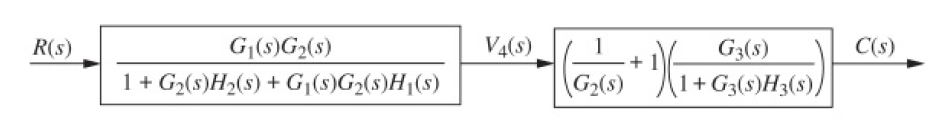
\includegraphics[width=1.1\linewidth]{Figuras/Ch09/fig30.PNG}}
}

\frame{
\frametitle{Exemplo $\#05$ - redução de diagrama de blocos}
\begin{block}{Resolução}
\begin{itemize}
    \item Finalmente, multiplique os dois blocos em \textbf{cascata} e obtenha o resultado final.
\end{itemize}
\end{block}
\vspace{0.3cm}
\centerline{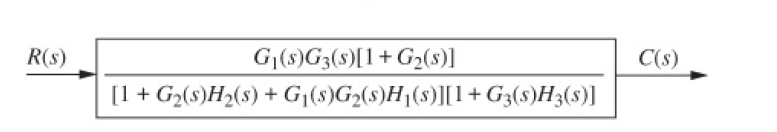
\includegraphics[width=0.9\linewidth]{Figuras/Ch09/fig31.PNG}}
}

\frame{
\frametitle{Exercícios}
\begin{block}{}
01. Revisite todos os exercícios propostos (final de capítulo) de modelagem de sistemas mecânicos de translação, sistemas mecânicos de rotação e sistemas elétricos; e desenhe todos os possíveis diagramas de blocos, a partir das EDOs. 

\vspace{0.5cm}

02. Para cada um dos dois sistemas abaixo, simplifique o diagrama de blocos e, então, obtenha a função de transferência de malha fechada.
\end{block}
\vspace{0.3cm}
\centerline{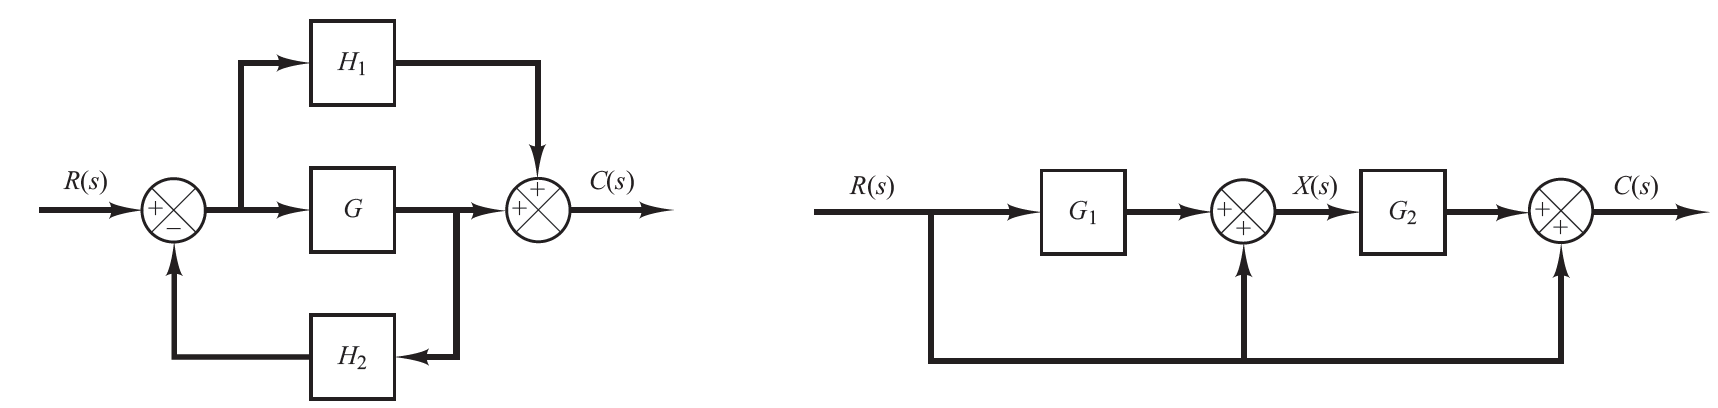
\includegraphics[width=1.1\linewidth]{Figuras/Ch09/fig32.PNG}}
}

\frame{
\frametitle{Referências e exercícios complementares}
\begin{itemize}
\item  NISE, Norman S. Engenharia de Sistemas de Controle, 7 ed. LTC, 2017.
\end{itemize}
\centering{\alert{Página 230 - \textbf{Capítulo 5}}} \\
\vspace{0.4cm}
\begin{itemize}
\item OGATA, Katsuhiko. Engenharia de Controle Moderno, 5 ed. Pearson, 2010.
\end{itemize}
\centering{\alert{Página 52 - \textbf{Capítulo 2}}} \\
}